\documentclass[a4paper,11pt,oneside,reqno,table]{book}


% extbook - a class for text bigger than 12pt
%\documentclass[a4paper,14pt,twoside,openright,reqno,table]{extbook}

% Options in detail:
% openany - allows chapter and similar openings to occur on left hand pages
% openright - allows chapter and similar openings to occur on right hand pages
% fleqn  - left-alignment of formulas
% leqno - labels formulas on the left-hand side instead of right
% reqno - labels formulas on the right-hand side
% draft - in draft mode the figures are not loaded, useful for speeding up typesetting
% onecolumn or twocolumn
% oneside (default for article and report)
% twoside (default for book)
% table  --> to avoid the message: package xcolor has already been loaded ...

\usepackage{packages}
% Almost all the settings are defined in packages.sty

% Put a grey textual watermark on document pages (PS mode only)
%\usepackage[italian,light,first,bottomafter]{draftcopy}

% Put a grey textual watermark on document pages (PDF mode)
%\usepackage{draftwatermark}
% If you want to change the default DRAFT text
%\SetWatermarkText{DRAFT}
% If you want to change the default grey color of the text
%\SetWatermarkColor{red}

%%%%%%%%%%%%%%%%%%%%%%%%%%%%%%%%%%%%%%%%%%%
%   DOCUMENT: an ordered list of files    %
%             that you can include or not %
%             in your document            %
%%%%%%%%%%%%%%%%%%%%%%%%%%%%%%%%%%%%%%%%%%%
\begin{document}

% FRONTISPIECE %
\begin{titlepage}
% \changepage with:
% {textheight}{textwidth}{evensidemargin}{oddsidemargin}{columnsep}
% {topmargin}{headheight}{headsep}{footskip}
\changepage{}{}{}{-7.5 mm}{}{}{}{}{}
%\InMiddlePage {copertina}

\begin{center}
%\includegraphics [width=.15\columnwidth, angle=0]{unipd1}\\ % height
{\LARGE \bf \scshape Universit\`a Politecnica delle Marche}\\
\vspace{0.2cm}
{\Large \bf \scshape Facolt\`a di Ingegneria}\\
\vspace{0.2cm}
{\Large Dipartimento di Ingegneria dell'Informazione}\\
\vspace{0.2cm}
{\large Corso di Laurea in Ingegneria Informatica e dell'Automazione}\\

\rule{150mm}{.2mm}


\vspace{10mm}

\begin{figure}[h!]
	\centering
	
\includegraphics[width=3.5cm]{logo.png}
\end{figure}

\vspace{10mm}

\textbf{ \large \scshape Tesi di Laurea}

\vspace{8mm}

\Large{\bf Titolo della tesi in italiano}

\vspace{7mm}

\Large{\bf Titolo della tesi in inglese}

\end{center} 	
\vspace{20mm} 	
\begin{center}
\begin{tabular}{lcl}
	{\large Relatore} & \ \hskip 6cm \ & {\large Candidato} \\
	\ & \ & \\
	{Dott. Enrico Corradini} \ & \ & {Nome Cognome Candidato} \\
	\ & \ & \ \\
	\ & \ & \ \\
	
\end{tabular}

\vspace{12mm}

\rule{150mm}{.2mm}

\textbf{\scshape Anno Accademico 2020-2021}
\end{center} 	
\end{titlepage}



%% FRONTMATTER %%
% The pages inside of frontmatter are in Roman numerals and the chapters will not have numeration
\frontmatter

% CREDITS %
\begin{titlepage}

\nonumber
\null \vspace {\stretch{1}}
	\begin{flushright}
%	\begin{verse}
\textit{Frase da citare (se si vuole)} \\[5mm]
%	\end{verse}
	Autore della citazione
	\end{flushright}
\vspace{\stretch{2}}\null

\end{titlepage}
\cleardoublepage

% ABSTRACT %
%\selectlanguage{italian}
\begin{abstract}

Questo è l'abstract della tesi.
\\[1cm]
\textbf{Keyword}: Queste sono le keywords della tesi
\end{abstract} 

\selectlanguage{italian}

% TOCs %
%% To help hyperref to jump to the correct page
\phantomsection
\addcontentsline{toc}{chapter}{Indice}
\tableofcontents
\clearpage

\tableofcontents   
\listoffigures
\listoftables


% GLOSSARY
%\cleardoublepage
% To help hyperref to jump to the correct page
\phantomsection
% To add the Glossary in the table of contents
\addcontentsline{toc}{chapter}{Glossario}
% Prints the glossary
\printglossary
% In order to update the glossary you have to execute:
% makeindex -s main.ist -t main.alg -o main.acr main.acn
% to insert an item in the document:
% \newglossaryentry{item_label}{name={item}, description={description}}
% if it doesn't appear you have to initialize it:
% \glsadd{item_label}
% or if it is called again in the following text:
% \gls{item_label}

% SYMBOLS %
%\cleardoublepage
% To help hyperref to jump to the correct page
\phantomsection
% To add the Index of Symbols in the table of contents
\addcontentsline{toc}{chapter}{Elenco dei simboli}
% Prints the Index of Symbols
\printglossary[type=\acronymtype,title=Elenco dei simboli]
% In order to update the symbols you have to execute:
% makeindex -s main.ist -t main.glg -o main.gls main.glo
% to insert an item in the document::
% \newacronym{item_label}{name={item}, description={description}}
% if it doesn't appear you have to initialize it:
% \glsadd{item_label}
% or if it is called again in the following text:
% \gls{item_label}

%% MAINMATTER %%
% The pages inside of mainmatter are in Arabic numerals and the chapters will have numeration
\mainmatter

%\part{Studio iniziale}
\phantomsection
\addcontentsline{toc}{chapter}{Introduzione}
\chapter*{Introduzione}
\markboth{Introduzione}{}

Questa è l'introduzione della tesi.

Specificare i capitoli della tesi:
\begin{itemize}
	\item Capitolo 1, descrizione.
	\item Capitolo 2, descrizione.
	\item ecc...
\end{itemize}

\chapter{Esempio di capitolo} %\label{1cap:spinta_laterale}

\begin{preamble}
{\em Riassunto del capitolo. In questo capitolo...}
\end{preamble}

\section{Sezione 1}
Sezione 1 del capitolo con Figura \ref{fig:esempio}

\begin{figure}[h]
	\centering
	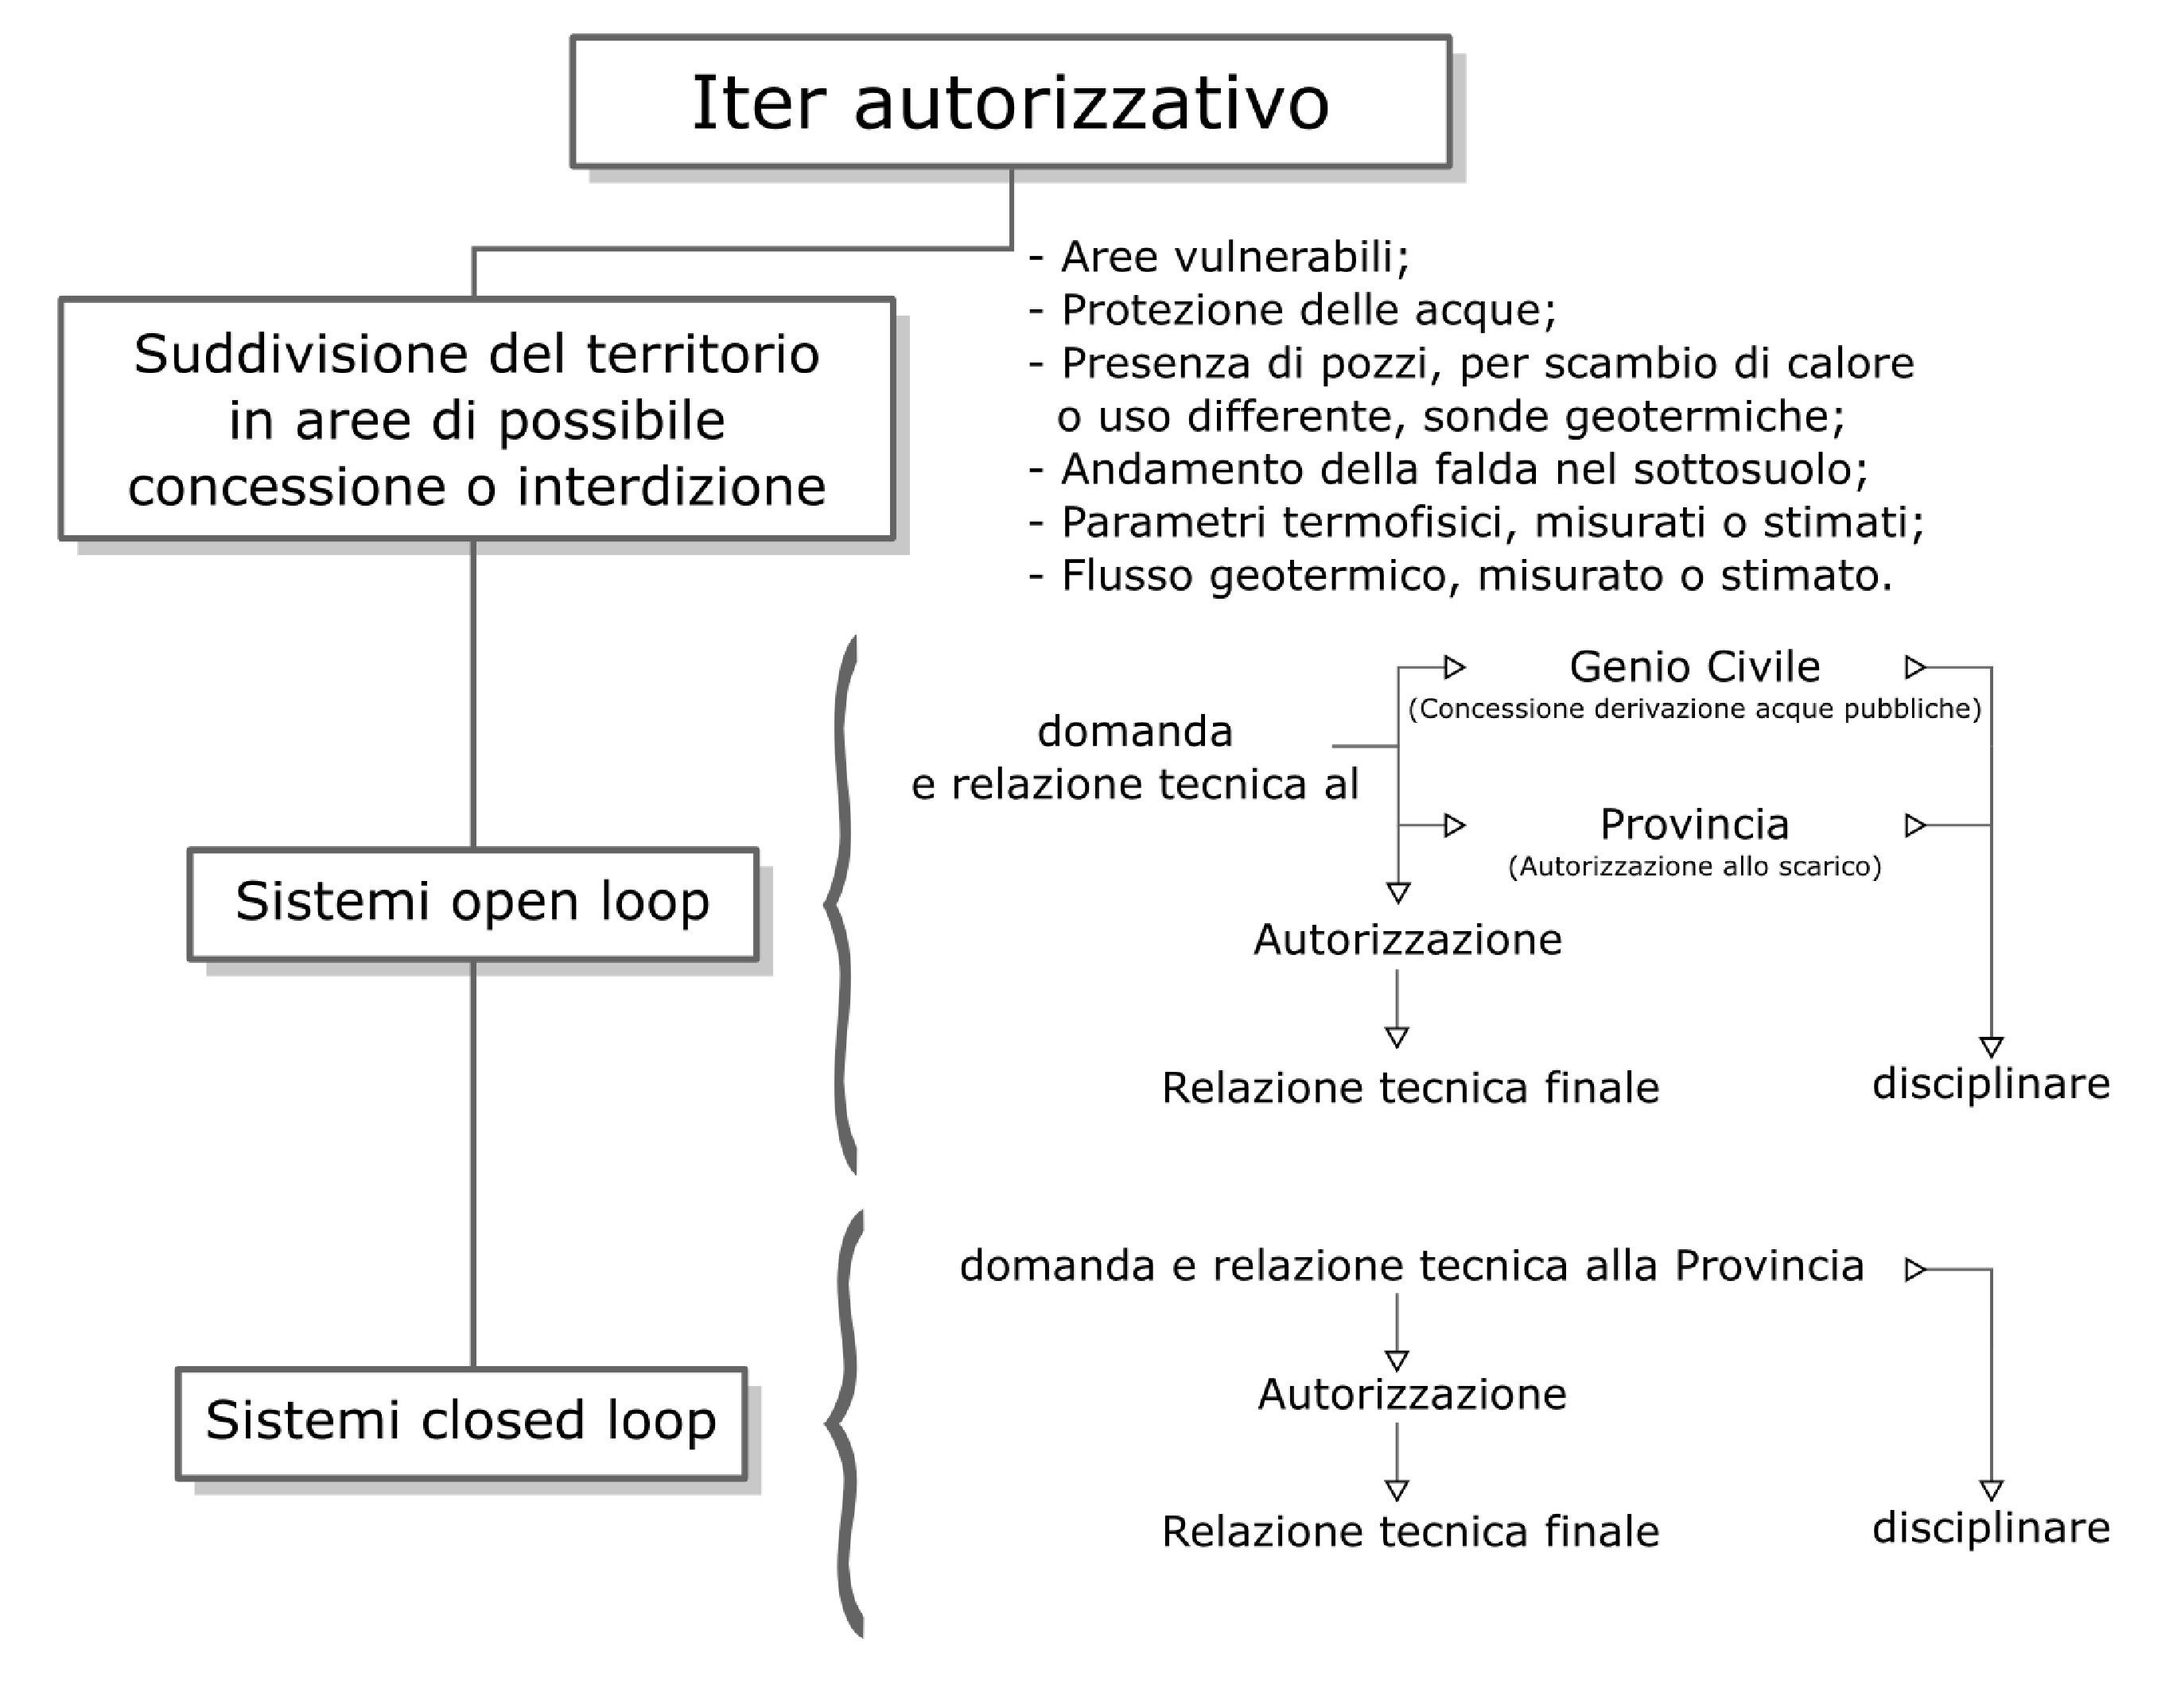
\includegraphics [width=.95\columnwidth, angle=0]{iter_autorizzativo} % height
	\caption{Figura Esempio}
	\label{fig:esempio}
\end{figure}

\subsection{Sezione 2}
Sezione 2 con sottosezione.

\subsection{Sottosezione 2.1}
Sottosezione con Tabella \ref{tab:esempio}.

\begin{table}[h]
\centering
\rowcolors{2}{gray!25}{}
\begin{tabular}{lll}
\toprule
{\bf Valore 1} & {\bf Valore 2} & {\bf Valore 3} \\
\midrule
10	& 20 & 30 \\
40 & 50 & 60 \\
\bottomrule
\end{tabular}
\caption{Tabella di esempio}
\label{tab:esempio}
\end{table}

% APPENDICES
%\appendix
%\include{appendix1/appendix1}
%\include{appendix2/appendix2}

%% BACKMATTER %%
% The pages inside of backmatter are in Arabic numerals and the chapters will not have numeration
\backmatter

% BIBLIOGRAPHY WITH BIBTEX %
%*******************************************************
% Bibliography
%*******************************************************
\cleardoublepage
\phantomsection
\addcontentsline{toc}{chapter}{\bibname}
\nocite{*}
% The style can be: classic, plainnat, abbrvnat or unsrtnat
\bibliographystyle{classic}
\bibliography{bibliography}
%

\vspace{2.5cm}
\begin{Large}Websites consulted\end{Large}
\begin{itemize}
\item Nome website	-- \url{www.url.com}
\item Altri se esistono
\end{itemize}


% All the sources are described in a file named bibliography.bib
% if you want to cite one in the text:
% \citep{label}
% In order to update the bibliography you have to execute:
% bibtex main (without ".tex")

\chapter*{Ringraziamenti}
\addcontentsline{toc}{chapter}{Ringraziamenti}
\markboth{Ringraziamenti}
\emph{Ringraziamenti} 

% INDEX %
%\cleardoublepage
% To help hyperref to jump to the correct page
\phantomsection
% To add the Index in the table of contents
\addcontentsline{toc}{chapter}{Indice analitico}
% Prints the Index
\printindex
% To add an item in it, write the \index{WORD} after the word to highlight:
% WORD\index{WORD}
% In order to update the Index you have to execute:
% makeindex main (without ".tex")

% A typical session involving a bibliography, an index and son on would require:
% pdflatex main
% makeindex -s main.ist -t main.alg -o main.acr main.acn
% makeindex -s main.ist -t main.glg -o main.gls main.glo
% bibtex main
% pdflatex main
% pdflatex main
% makeindex main
% makeindex -s main.ist -t main.alg -o main.acr main.acn
% makeindex -s main.ist -t main.glg -o main.gls main.glo
% pdflatex main
% pdflatex main
\end{document}